\section{Demystifying AI Agents}
\label{sect:char_workflow}

\sect{sect:workflow_call_count} first examines an agent's \emph{single}-request execution, followed by a detailed exploration of the LLM inference and tool-calling characteristics of agents in \sect{sect:char_llm_inference}. Lastly, \sect{sect:char_serving} shifts the focus to the serving environment of agentic systems where \emph{multiple} requests are handled concurrently, identifying system-level bottlenecks and scalability issues that emerge in agent deployment.
 

\subsection{Overall Workflow of AI Agents}
\label{sect:workflow_call_count}

\begin{figure}[t!] \centering
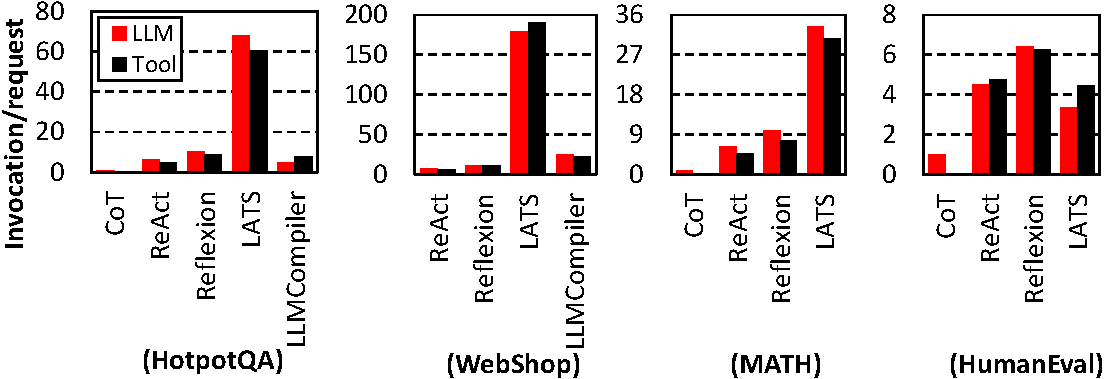
\includegraphics[width=0.48\textwidth]{./fig/workflow_call_count}
\vspace{-0.4em}
\caption{
Average number of LLM and tool invocations per request.
}
\label{fig:workflow_call_count}
\end{figure}

{\bf Effect of LLM and tool calls on latency.}
\fig{fig:workflow_call_count} shows the average number of LLM and tool invocations per request across benchmarks. While CoT performs only a single LLM inference per request, tool-augmented agentic systems require significantly more LLM calls, averaging 9.2 times more than CoT. Among these, LATS exhibits the highest LLM invocation count, with an average of 71.0 LLM calls per request. This is primarily due to its use of tree search, which explores multiple reasoning branches (i.e., child nodes) by issuing separate LLM inferences for each one when expanding a tree node.

\begin{figure}[t!] \centering
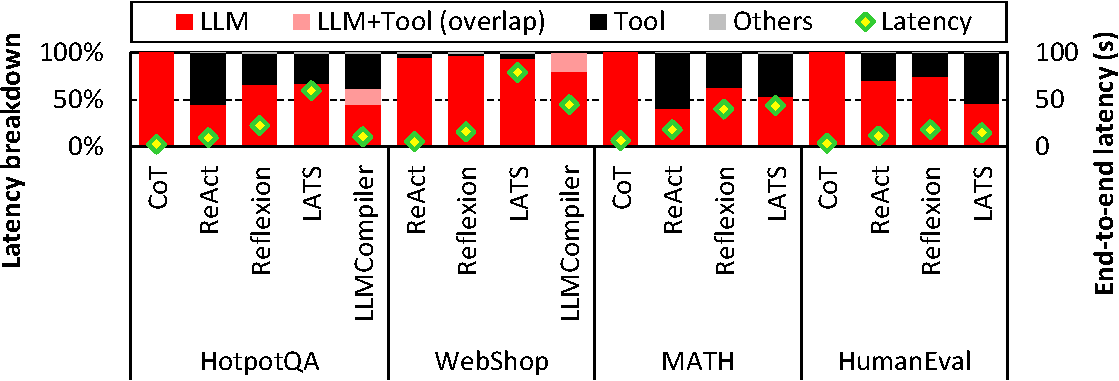
\includegraphics[width=0.48\textwidth]{./fig/workflow_latency_breakdown}\\
\vspace{-0.4em}
\caption{
Latency breakdown of agents (left axis, bar graph) and their end-to-end latency for processing a single request (right axis, diamond marker). The pink bars represent phases where LLM and tool execution latencies overlap, as observed in LLMCompiler, which asynchronously executes tools during plan generation.}
\label{fig:workflow_latency_breakdown}
\vspace{-0.9em}
\end{figure}

\fig{fig:workflow_latency_breakdown} presents the end-to-end latency and the latency breakdown of each agent's execution. While most agents exhibit a similar number of LLM and tool calls per request (\fig{fig:workflow_call_count}), the latency contribution from tool calls varies significantly depending on the workload. This discrepancy is primarily due to differences in the underlying tool execution latencies. For example, WebShop uses lightweight tools that interact with locally hosted webpages, resulting in tool latencies as low as 20 ms per call. In contrast, HotpotQA relies on the Wikipedia API, where individual calls take an average of 1.2 seconds. As a result, tool execution dominates the overall latency breakdown in this case. 

On average, LLM inference and tool execution account for 69.4\% and 30.2\% of total latency, respectively. Both stages contribute significantly to overall latency, but they are difficult to overlap due to their sequential dependency. Specifically, the LLM output is needed to determine which tool to invoke along with the required arguments. Conversely, the next LLM invocation typically relies on the observation returned by the tool. Although LLMCompiler attempts to mitigate this dependency by streaming intermediate plans to the scheduler for asynchronous execution of tool calls (thus concurrently executing it with planning), the observed overlap accounts for only 18.2\% of total latency.


\begin{figure}[t!] \centering
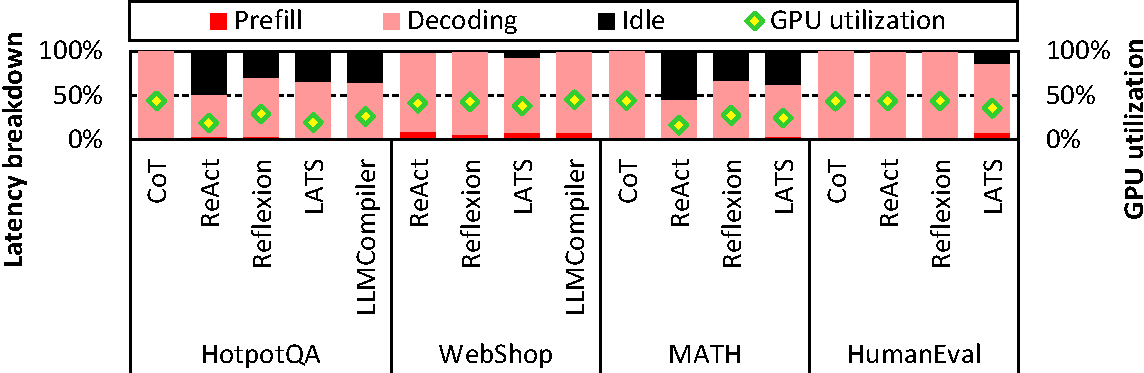
\includegraphics[width=0.48\textwidth]{./fig/workflow_gpu_utilization}\\
\vspace{-0.4em}
\caption{
Breakdown of GPU runtime by usage (left axis, bar graph) and the resulting average GPU utilization (right axis, diamond marker). GPU utilization is measured as the fraction of actively used GPU cores, using NVIDIA's DCGM~\cite{dcgm}.
}
\label{fig:workflow_gpu_utilization}
\vspace{-1em}
\end{figure}

{\bf Agentic workflow's effect on GPU compute utility.}
\fig{fig:workflow_gpu_utilization} breaks down the GPU runtime by usage and reports the resulting average GPU utilization when handling a single request. Although this setup assumes the processing of a single agent task, concurrent LLM calls can be opportunistically batched to improve GPU utilization, whenever possible, to more efficiently execute agents such as LATS. Unlike CoT, which performs a single LLM inference without external interaction, it is possible for agents to experience longer GPU idle periods due to tool execution. The duration of these idle periods depends on the tool’s latency and whether it leverages the GPU. In WebShop, the tool interacts with locally hosted synthetic web pages, resulting in very short tool latencies (\fig{fig:workflow_latency_breakdown}), so agents do not experience notably higher GPU idle time (i.e., lower GPU utilization). HumanEval exhibits longer tool execution times (\fig{fig:workflow_latency_breakdown}), but the proportion of GPU idle time remains minimal because the tool it calls (which is the test generation tool) utilizes the GPU for LLM execution. In contrast, HotpotQA and MATH employ tools that operate on local CPUs or external systems, leading to substantial GPU idle periods that account for up to 54.5\% of total execution time, resulting in significantly lower GPU utilization compared to CoT.
When the GPU is executing the LLM, its activity can be further divided into the prefill and decode stages, which account for 4.7\% and 74.1\% of the GPU’s execution time, respectively. As noted in ~\cite{sarathi,Leviathan2023SpecDecode,medusa,ainslie2023gqa}, the decode stage is known to be memory-bound. Consequently, the large fraction of time spent in the decode stage further contributes to the underutilization of GPU resources.


Because the sequential dependency between LLM inference and tool calls limits parallel execution opportunities within a single request (i.e., intra-request parallelism), improving overall resource utilization requires leveraging \emph{inter}-request parallelism. We explore this direction in \sect{sect:char_serving}, where we discuss the implications of serving AI agents over multiple queries with LLM request batching~\cite{orca,vllm,vllm_repo}.


\begin{figure}[t!] \centering
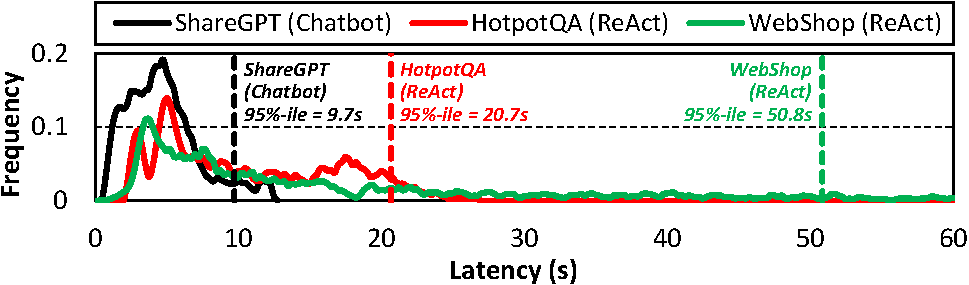
\includegraphics[width=0.48\textwidth]{./fig/latency_distribution_new}
\vspace{-0.4em}
\caption{
End-to-end latency distribution of a non-agentic ShareGPT workload and ReAct-based agents with HotpotQA and WebShop workloads. Latency is measured while processing one request at a time, with prefix caching enabled.
}
\label{fig:latency_distribution}
\end{figure}

\textbf{End-to-end latency distribution of AI agents.}
\fig{fig:latency_distribution} compares the end-to-end latency distributions of a conventional, non-agentic LLM service using ShareGPT and a ReAct-based agent system using HotpotQA and WebShop.
The ShareGPT dataset represents a typical chatbot workload, where each response is generated by a single LLM inference. 
As shown, this results in a relatively low and consistent latency distribution, with most responses completing within 9.7 seconds. In contrast, the ReAct-based agent exhibits a much broader latency distribution with a heavier tail, due to its multi-step reasoning and reliance on external tools. Because the number of reasoning steps and tool calls varies across requests in agents, the associated computational demands also fluctuate. Consequently, there is significant variance in latency across queries targeting agents. 


\subsection{LLM Inference and Tool-Calling Characteristics}
\label{sect:char_llm_inference}

This section further analyzes the behavior of agentic systems by characterizing the properties of LLM inference and tool calls within the AI agent in greater detail.

\textbf{Breakdown of input and output tokens in LLM inference.} \fig{fig:token_breakdown} presents the token count distribution across different AI agents. \textit{Instruction} tokens define the agent’s role and objective within the task, while \textit{Few-shot} tokens provide in-context examples that guide the agent’s behavior. \textit{User} tokens represent user queries. \textit{LLM history} and \textit{Tool history} tokens consist of accumulated outputs from previous LLM inferences and tool responses across iterations. \textit{Output} tokens are generated at each LLM inference step, while the remaining tokens collectively make up the input prompt.


\begin{figure}[t!] \centering
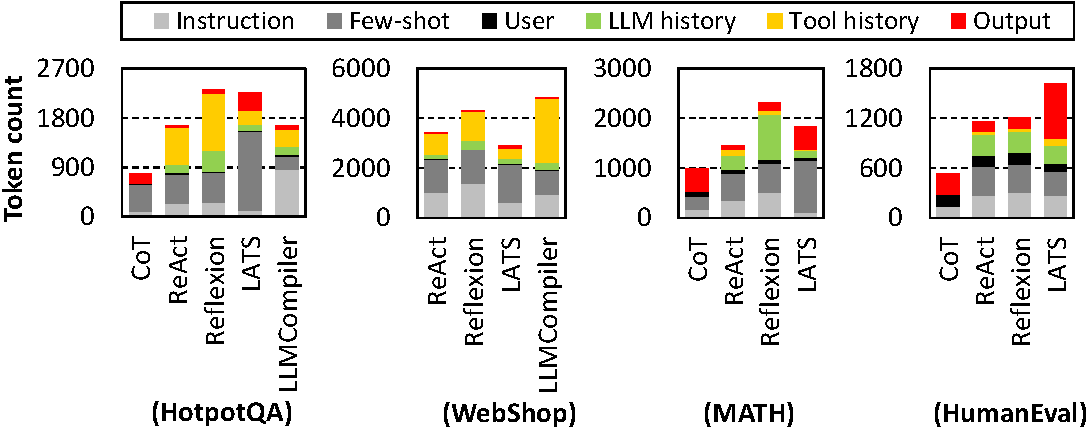
\includegraphics[width=0.48\textwidth]{./fig/token_breakdown}\\
\caption{
Breakdown of input and output tokens in LLM inference. \emph{Instruction} and \emph{Few-shot} (light and dark gray) represent input tokens that are statically fixed as part of the initial prompt to the LLM. \emph{User} (black) denotes input tokens provided by the user as part of the query. \emph{LLM history} (green) and \emph{Tool history} (yellow) represent tokens accumulated from previous LLM outputs and tool responses, respectively, which are then included as input tokens during the next LLM call. \emph{Output} (red) refers to tokens generated by each LLM call.}
\label{fig:token_breakdown}
\vspace{-1em}
\end{figure}

Compared to CoT, AI agents generally have longer input tokens. This is because their inputs include additional elements such as agent role-aligned instructions (e.g., LLMCompiler requires instructions to generate a structured plan) and the accumulated context of previous LLM and tool interactions. For output tokens, each LLM call in agent workflows often generates fewer tokens than CoT, except for LATS. This is because agents typically decompose a single task into multiple steps, distributing the overall output across several LLM calls. In contrast, LATS often generates much longer outputs than CoT due to its workflow, where a single LLM call produces multiple candidate samples to expand the tree node.


Token usage patterns also vary depending on the task workload. In knowledge-intensive tasks such as HotpotQA and decision-making tasks like WebShop, tool calls often return large responses (e.g., the full content of a webpage) resulting in longer tool history tokens. In contrast, tasks that rely more heavily on internal reasoning, such as MATH and HumanEval, tend to produce longer LLM-generated outputs, leading to larger LLM history tokens.


Although the ratio of LLM and tool history tokens varies across workloads, most benchmarks exhibit substantial growth in input history over multiple iterations. An exception is LATS, which includes only the path from the root to the current node, rather than concatenating all prior interaction histories. 
In the case of HotpotQA, for instance, initial inputs are typically around 1,000 tokens, but the input size increases to 3–4$\times$ as prior LLM outputs and tool responses are appended to the input context of subsequent LLM calls. Because histories accumulate sequentially, consecutive LLM calls share common prefixes in their input contexts. These long input contexts result in high KV cache usage per request and considerable prefix overlap across iterations. This behavior presents an opportunity to improve GPU compute and memory efficiency through \emph{prefix caching}~\cite{vllm}, as detailed below.


\textbf{Effect of prefix caching on AI agent's compute efficiency.}
Building on the token-level analysis above, we now turn to system-level characteristics, starting with GPU compute efficiency. AI agent workloads involve multiple iterative LLM calls, where a large portion of the input context is reused at each step. Prefix caching leverages this shared prefix to skip redundant computation during the prefill phase by reusing previously cached key-value (KV) pairs.

\begin{figure}[t!] \centering
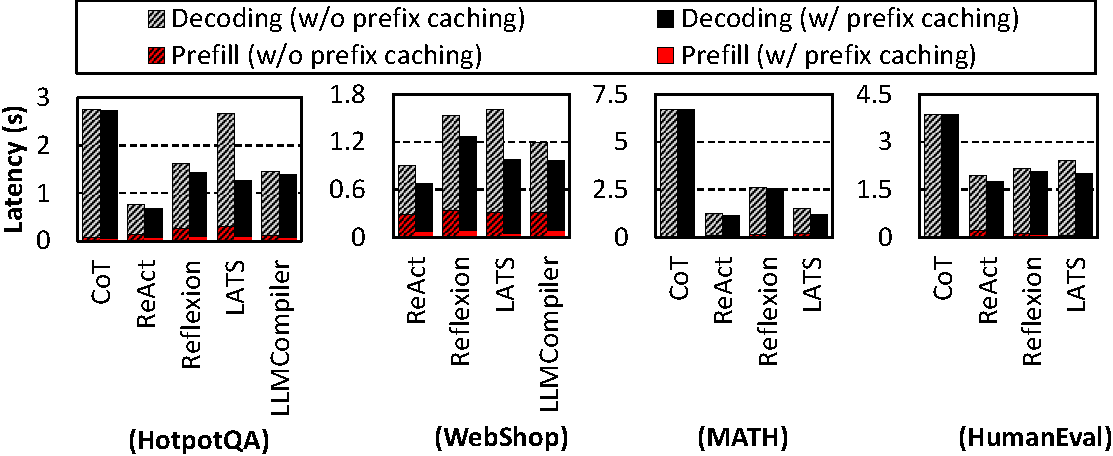
\includegraphics[width=0.48\textwidth]{./fig/workflow_llm_latency_and_breakdown}\\
\vspace{-0.4em}
\caption{
Inference latency with(out) prefix caching and its breakdown.}
\label{fig:workflow_llm_latency_and_breakdown}
\vspace{-1em}
\end{figure}

\fig{fig:workflow_llm_latency_and_breakdown} shows LLM inference latency and its proportion of prefill and decoding latency, with and without prefix caching. For CoT, LLM inference occurs only once per request, and the shared prefix across inferences is minimal. Moreover, CoT typically generates a relatively large number of output tokens, making decoding the dominant contributor to latency. In contrast, AI agents operate iteratively and accumulate long input contexts due to interaction histories. As a result, prefix caching reduces prefill latency by an average of 60.1\%, demonstrating its effectiveness in improving compute efficiency by avoiding redundant computations through prefix reuse.
Beyond the prefill phase, prefix caching can also indirectly improve decoding efficiency. In systems that execute multiple parallel LLM calls, decoding may be stalled by ongoing prefill operations. By reducing prefill latency, prefix caching shortens this blocking period, thereby enabling faster decoding and explaining the larger speedup observed in LATS.


Overall, the impact of prefix caching on end-to-end LLM inference latency varies by workload type. While CoT workloads benefit less due to their decoding-dominant property, agentic workloads experience an average 15.7\% reduction in end-to-end latency due to the accumulation of long input contexts over iterative steps. While this per-request improvement may seem modest, the reduction in prefill time can significantly alleviate system-level bottlenecks. In token-level schedulers like vLLM, long prefill phases can delay the scheduling of concurrent requests. By shortening these phases, prefix caching can improve scheduling efficiency and increase overall system throughput. This effect is examined further in \sect{sect:char_serving} (\fig{fig:serving_prefix_caching}).


\textbf{Effect of prefix caching on AI agent's memory efficiency.}
We now discuss the effect of prefix caching on GPU memory requirements by measuring the average GPU memory required to store the KV cache. On average, tool-augmented AI agents consume 3.0$\times$ more memory per request than CoT, and up to 5.4$\times$ more in the worst case. This overhead arises from the iterative nature of agent workflows, where each LLM call appends intermediate reasoning steps and tool responses to the context, resulting in a longer input for each LLM inference.


These results highlight the need for memory optimization in AI agent workloads, with prefix caching serving as a key technique for reducing GPU memory usage. In LATS, multiple LLM inferences are issued in parallel to evaluate several child nodes simultaneously during tree expansion. Without prefix caching, each of these parallel calls creates its own KV cache, resulting in significant memory overhead due to redundancy. With prefix caching, the shared prefix across these parallel calls can be reused, reducing memory requirements by an average of 64.8\% in LATS. For other agents, where all LLM calls are invoked sequentially, prefix caching does not reduce memory usage \emph{within a single request}, since the KV cache cannot be shared across LLM calls. However, in serving scenarios with concurrent requests, prefix caching can significantly improve memory efficiency by reusing the KV cache across requests. We further explore this serving-level memory efficiency in \sect{sect:char_serving} (\fig{fig:serving_memory_efficiency}).


\begin{figure}[t!] \centering
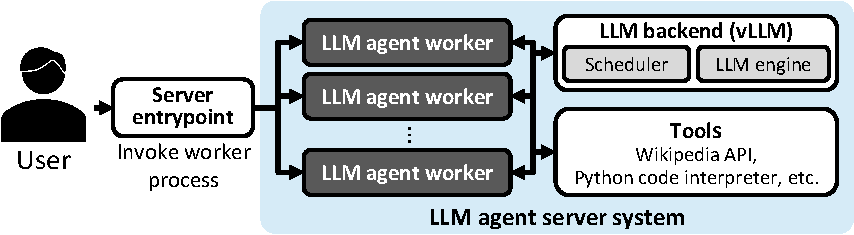
\includegraphics[width=0.47\textwidth]{./fig/serving_overview}\\
\vspace{-0.4em}
\caption{
High-level overview of our AI agent serving system. 
}
\label{fig:serving_overview}
\vspace{-0.6em}
\end{figure}


\subsection{AI Agent Serving Characteristics}
\label{sect:char_serving}

So far, our characterization has focused on the behavior of AI agents when servicing a single query for a specific task. In this section, we shift our attention to system-level properties of AI agent serving environments, analyzing scenarios where multiple requests are routed to the server and can be processed concurrently for high serving throughput. Unlike static reasoning models that process a user request with a single LLM inference step, AI agents perform multiple reasoning steps iteratively, introducing new challenges for efficient serving.

To examine the characteristics of AI agent serving, we implement an agent serving system, as illustrated in \fig{fig:serving_overview}. When a user sends a request to the agent server’s entry point, each worker processes the request according to the agent’s workflow. Depending on the current step of the task, a worker either sends a request to the LLM inference server or executes a tool. Tool execution may occur locally (e.g., code interpreters, custom functions) or involve external resources (e.g., web search, API calls). Each worker operates asynchronously, and LLM inference requests from multiple workers can be batched at the LLM backend (e.g., vLLM) for high-throughput processing using continuous batching~\cite{orca,vllm}. We adopt vLLM’s default first-come-first-served (FCFS) scheduler in the LLM inference backend. To simulate realistic traffic, input queries to the agent server are randomly sampled and issued to the server following a Poisson arrival distribution~\cite{mlperf_datacenter}.




\textbf{Importance of concurrent request scheduling.} 
Before comparing the AI agent serving against the conventional chatbot (ShareGPT) serving, we first highlight the importance of concurrently servicing AI agent requests. When ReAct agents are executed \emph{sequentially}, the average latency is 9.6 seconds for HotpotQA and 5.3 seconds for WebShop, limiting throughput to 0.10 and 0.19 queries per second (QPS), respectively. With \emph{concurrent execution}, throughput improves to 2.6 and 1.2 QPS for HotpotQA and WebShop (\fig{fig:serving_prefix_caching}), respectively, achieving 25$\times$ and 6.2$\times$ gains at the cost of a 2.1$\times$ increase in average latency. The greater throughput gain in HotpotQA comes from its longer tool latency, which causes the GPU to remain idle for extended periods. These idle intervals can be effectively utilized by servicing other requests, enabling higher concurrency and throughput. 


\begin{figure}[t!] \centering
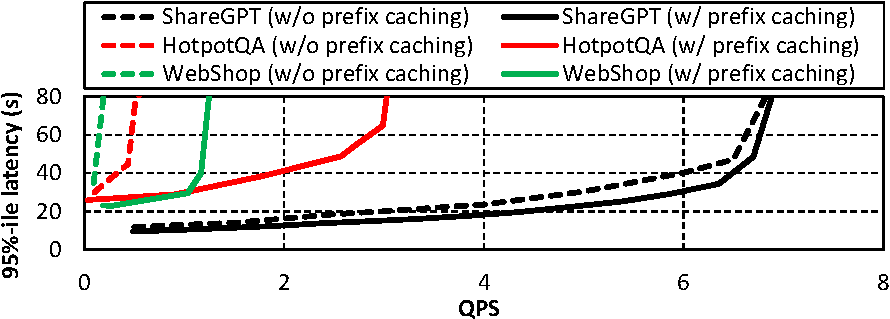
\includegraphics[width=0.48\textwidth]{./fig/serving_prefix_caching_new}\\
\vspace{-0.4em}
\caption{ 
95th percentile latency for chatbot (ShareGPT) and ReAct-based AI agents (HotpotQA and WebShop) as QPS rates increase, with (solid line) and without (dashed line) prefix caching enabled.
}
\label{fig:serving_prefix_caching}
\end{figure}

\textbf{Comparison with conventional static reasoning LLM services.}
We now compare an AI agent serving with a conventional LLM serving scenario, represented by the chatbot (ShareGPT) workload. ShareGPT, a typical single-turn LLM service, processes user queries in a single inference pass. \fig{fig:serving_prefix_caching} shows the changes in end-to-end tail latencies for chatbot (ShareGPT) and ReAct-based AI agent (HotpotQA and WebShop) workloads as input QPS to the server increases. The peak throughput is measured as the maximum sustainable QPS at the knee of the tail latency curve. As depicted, the peak throughput of ReAct is significantly lower than that of ShareGPT. While ShareGPT can sustain up to 6.4 QPS, ReAct supports only 2.6 QPS on HotpotQA and 1.2 QPS on WebShop, even with prefix caching enabled. This limitation stems from ReAct’s multi-step reasoning, where each request involves multiple LLM calls and tool interactions, significantly increasing latency. 



\textbf{Effect of prefix caching on AI agent serving throughput.}
Prefix caching is an important system-level optimization that reduces redundant computation during the prefill phase of LLM inference by reusing previously computed key-value (KV) caches. While its impact on the latency of individual LLM calls is modest (\fig{fig:workflow_llm_latency_and_breakdown}), it can substantially improve throughput and serving efficiency for AI agents.


\fig{fig:serving_prefix_caching} compares the effect of prefix caching on chatbot (ShareGPT) and agentic (ReAct) workloads. ShareGPT shows only a modest 1.03$\times$ throughput improvement, as it performs a single LLM call per request with minimal repetition. In contrast, ReAct benefits significantly, achieving an average 5.62$\times$ increase in throughput. This is because agent workloads involve multiple LLM calls per request, amplifying the benefits of avoiding redundant prefill operations.


The performance gap is further explained by token-level batching systems such as vLLM. Without prefix caching, long prefill stages occupy the GPU and block decoding for other requests, leading to system-wide queuing delays. This bottleneck is particularly problematic for AI agents, where repeated LLM calls per request exacerbate inter-request contention. As a result, prefix caching plays a critical role in mitigating these interference effects and improving overall serving efficiency, especially for agentic workloads.

\begin{figure}[t!] \centering
\vspace{-1em}
\captionsetup[subfloat]{captionskip=0.3em}
\subfloat[Average memory usage]{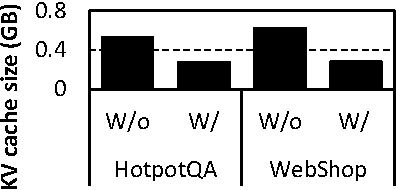
\includegraphics[width=0.22\textwidth]{./fig/serving_prefix_caching_kv_size_avg}}
\hspace{1em}
\subfloat[Maximum memory usage]{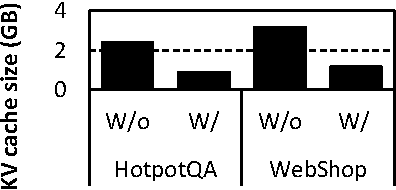
\includegraphics[width=0.22\textwidth]{./fig/serving_prefix_caching_kv_size_max}}
\caption{
(a) Average and (b) maximum memory used for KV caches, with and without prefix caching. Evaluation is conducted at 0.2 QPS (HotpotQA) and 0.1 QPS (WebShop) data points using ReAct.
}
\label{fig:serving_memory_efficiency}
\vspace{-0.4em}
\end{figure}

\textbf{Effect of prefix caching on AI agent's memory usage.}
We now investigate the impact of prefix caching on GPU memory efficiency in AI agent serving, focusing specifically on its effect on key-value (KV) cache size, one of the most significant contributors to memory usage in LLM inference. \fig{fig:serving_memory_efficiency} shows the GPU memory consumption for KV cache allocation, with and without prefix caching enabled, under identical QPS conditions. With prefix caching enabled, the average and maximum KV cache memory usage decrease by 51.7\% and 63.5\%, respectively, indicating improved memory efficiency. This reduction arises from the ability of prefix caching to reuse key-value pairs of shared prefix tokens across multiple LLM invocations across AI agent requests. Thus, prefix caching not only improves compute efficiency by eliminating redundant prefill operations but also reduces the KV cache memory footprint, enabling more efficient utilization of GPU memory during AI agent serving.
